\section{Einleitung}
\label{sec:intro}

Ich supporte eine kleine WebSite
\htmladdnormallink{http://www.ich-bin-am-wandern-gewesen.de/}{http://www.ich-bin-am-wandern-gewesen.de/}
mit dem Thema Wanderungen. Unter anderem werden dort die Fotos von
unseren Wanderungen pr�sentiert. Leider funktioniert meine
MiniFestplatte nicht immer (Strom?!?, SDHC etc.\ldots) und deswegen
m�ssen \emph{meine} Wanderkameraden(Innen) mir die Fotos per Mail zu
kommen lassen. Und dies kann \textbf{sehr} m�hselig sein, je nachdem
wieviel MB der MailAccount erlaubt\ldots{} Darum habe ich meine
Java-Kenntnisse herausgekramt und sogar eine Oberfl�che
programmiert\footnote{Mir h�tte ja ein ANT-Script wirklich gereicht.}
und dieses Progr�mmchen m�chte ich im nachfolgenden erl�utern.

\section{Installation}
\label{sec:installation}

Man/frau benutze auf Windows das InstallerScript, bei Linux muss ich
entsprechendes noch umsetzen.

\section{Benutzung}
\label{sec:using}

\begin{figure}[H]
\begin{minipage}[t]{.45\textwidth}
\centering\leavevmode
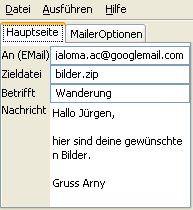
\includegraphics{images/oberflaeche}
\caption{Hauptseite}\label{fig:main:page}
\end{minipage}
\begin{minipage}[t]{.45\textwidth}
\centering\leavevmode
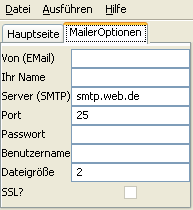
\includegraphics{images/oberflaeche_mailer}
\caption{Eingabe der Senderinformationen}\label{fig:mailer:page}
\end{minipage}
\end{figure}

Das Programm pr�sentiert sich mit einer einfachen Oberfl�chen
(Abb. \ref{fig:main:page}, \ref{fig:mailer:page}), in dieser hat der
Anwender seine Mail-Adresse (\code{Von (EMail)}), die Zieladresse
(\code{An (EMail)} sowie den Host einzugeben. Die Felder
\code{Zieldatei}, \code{Betrifft} und \code{Nachricht} sind
Themenbezogen schon vorbelegt. Nach der ersten Anwendung sollten die
Informationen sowieso abgespeichert werden, so dass beim n�chsten
Start die gespeicherten Werte angezeigt werden\footnote{Vorsicht: Das
Passwort wird nicht abgespeichert, da dies derzeit im Klartext in
dieser Datei landet!}.

Als n�chstes muss der \code{Host} eingetragen und der
\code{Port} ge�ndert werden.  Zur Sicherheit ist der \code{Benutzer}
und das \code{Passwort} einzugeben, der \code{Benutzer} kann
gleichbedeutend mit der Absenderadresse (\code{Von (EMail)} sein.

In dem Feld \code{Dateigr��e} kann die maximale Gr��e der EMail
eingestellt werden, der Wert wird als Megabyte-Angabe interpretiert.

\subsection{Versenden eines Bildverzeichnisse}
\label{sec:send:directory}
Wie versende ich jetzt ein Verzeichnis mit Bildern:
\begin{enumerate}
\item\label{it:an:email} \code{An (EMail)} eingeben.
\item\label{it:dest:file} \code{Zieldatei} bei Bedarf �ndern.
\item\label{it:subject} \code{Betrifft} nach Situation �ndern.
\item\label{it:message} \code{Nachricht} bearbeiten.
\item\label{it:von:email} Bei \code{Von (EMail)} deine EMail-Adresse
eingeben.
\item\label{it:smtp:server} Bei \code{Server (SMTP)} die Adressse wie
z.B. \texttt{smtp.web.de} eingeben.
\item\label{it:mail:port} \code{Port} eventuell �ndern. 
\item\label{it:passwort:user} \code{Passwort} und \code{Benutzername}
eventuell eingeben, der \code{Benutzername} kann durchaus von
\code{Von (EMail)} abweichen.
\item\label{it:file:size} \code{Dateigr��e} �ndern.
\item\label{it:save} \code{Datei $->$ Speichern}
\item\label{it:send:dir} \code{Ausf�hren $->$ Versende Verzeichnis},
Verzeichnis ausw�hlen und best�tigen und warten bis die Erfolgsmeldung
(Abb. \ref{fig:fertig}) erscheint.
\item Bei Erfolg beendet sich das Programm selber.
\end{enumerate}

\subsection{Versenden von Bilddateien}
\label{sec:send:files}
Beim Versenden von Bilder bitte die Schritte \ref{it:an:email} bis
\ref{it:save} in Abschnitt \ref{sec:send:directory} durchf�hren, anschliessend
\code{Ausf�hren $->$ Versende Dateien} anw�hlen, jetzt einzelne Bilder
anw�hlen, best�tigen und warten bis die Erfolgsmeldung
(Abb. \ref{fig:fertig}) erscheint, bei Erfolg beendet sich das
Programm selber.

\subsection{Fehlermeldungen}
\label{sec:error:messages}
Im nachfolgenden die m�glichen Fehlermeldungen:

\begin{figure}[H]
\begin{minipage}[t]{.45\textwidth}
\centering\leavevmode
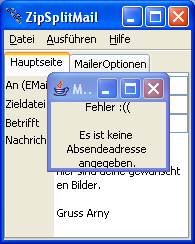
\includegraphics{images/fehler_keine_zieladresse}
\caption{Keine Zieladresse eingegeben}\label{fig:no:to:address}
\end{minipage}
%\end{figure}
%
%\begin{figure}[H]
\begin{minipage}[t]{.45\textwidth}
\centering\leavevmode
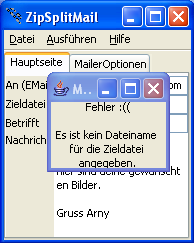
\includegraphics{images/fehler_keine_zieldatei}
\caption{Keine Zieldatei eingegeben}\label{fig:no:destfile}
\end{minipage}
\end{figure}

\begin{figure}[H]
%\begin{minipage}[t]{.45\textwidth}
\centering\leavevmode
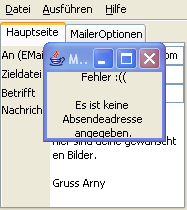
\includegraphics{images/fehler_keine_absendeadresse}
\caption{Keine Absenderadresse eingegeben}\label{fig:no:sender:address}
%\end{minipage}
\end{figure}
%
\begin{figure}[H]
\begin{minipage}[t]{.45\textwidth}
\centering\leavevmode
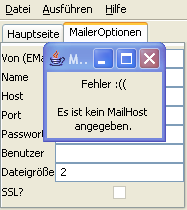
\includegraphics{images/fehler_kein_host}
\caption{Kein Mailhost eingegeben}\label{fig:no:mail:host}
\end{minipage}
%\end{figure}
%
%\begin{figure}[H]
\begin{minipage}[t]{.45\textwidth}
\centering\leavevmode
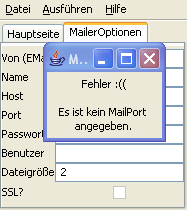
\includegraphics{images/fehler_kein_port}
\caption{Keinen Mailport eingegeben}\label{fig:no:mail:port}
\end{minipage}
\end{figure}

\begin{figure}[H]
\begin{minipage}[t]{.45\textwidth}
\centering\leavevmode
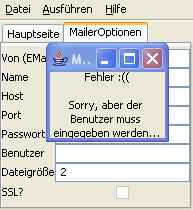
\includegraphics{images/fehler_kein_benutzer_wenn_passwort}
\caption{Keinen Benutzer eingegeben}\label{fig:no:user}
\end{minipage}
%\end{figure}
%
%\begin{figure}[H]
\begin{minipage}[t]{.45\textwidth}
\centering\leavevmode
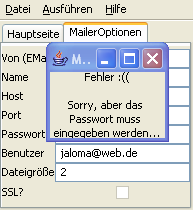
\includegraphics{images/fehler_kein_passwort_wenn_benutzer}
\caption{Kein Passwort eingegeben}\label{fig:no:password}
\end{minipage}
\end{figure}

\begin{figure}[H]
\centering\leavevmode
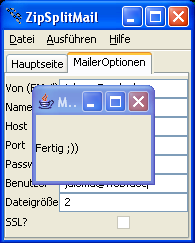
\includegraphics{images/fertig_meldung}
\caption{Es hat alles funktioniert}\label{fig:fertig}
\end{figure}

